\subsection{Introducción a las excepciones}
\subsection{Uso de try, except, else}
\subsection{Tipos de excepciones y manejo específico}
\begin{itemize}
    \item Ámbito local: Las variables declaradas dentro de una función tienen un ámbito local y solo son accesibles dentro de esa función.\\
\end{itemize}

    \begin{figure}[h]
        \centering
        \scalebox{0.35}{
        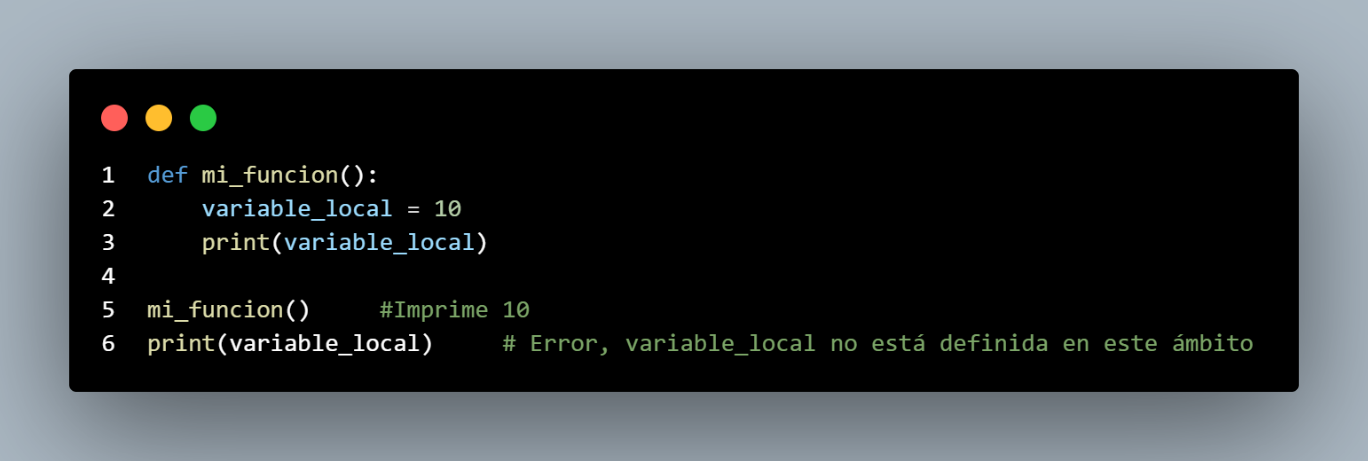
\includegraphics{Imagenes/fundamentos9.png}
        }
      \end{figure}


\begin{itemize}
    \item Ámbito Global: Las variables declaradas fuera de una función o declaradas como globales dentro de una función tienen un ámbito global y son accesibles desde cualquier parte del código.
\end{itemize}
    \begin{figure}[h]
        \centering
        \scalebox{0.35}{
        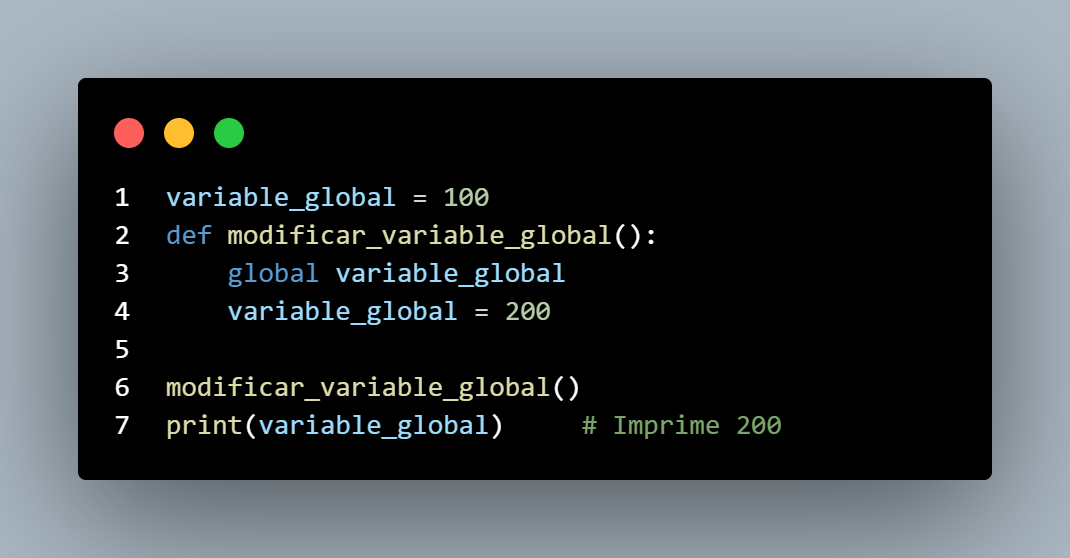
\includegraphics{Imagenes/fundamentos10.png}
        }
      \end{figure}
